\documentclass[12pt]{article}

% Mandatory Packages
\usepackage{amsmath}
\usepackage{amssymb}
\usepackage{amsthm}
\usepackage{geometry}
\usepackage{tikz}
\usetikzlibrary{arrows.meta, positioning, shapes, patterns}
\usepackage{mathrsfs}
\usepackage{mathtools}
\usepackage{xcolor}
\usepackage{hyperref}

% Geometry setup
\geometry{letterpaper, margin=1in}

% Theorem Environments
\newtheorem{theorem}{Theorem}[section]
\newtheorem{lemma}[theorem]{Lemma}
\newtheorem{proposition}[theorem]{Proposition}
\newtheorem{corollary}[theorem]{Corollary}
\theoremstyle{definition}
\newtheorem{definition}{Definition}[section]
\newtheorem{axiom}{Axiom}[section]
\newtheorem{example}{Example}[section]
\theoremstyle{remark}
\newtheorem{remark}{Remark}[section]

% Macros for Probability
\newcommand{\Pbb}{\mathbb{P}}
\newcommand{\Ebb}{\mathbb{E}}
\newcommand{\Fcal}{\mathcal{F}}
\newcommand{\Bcal}{\mathcal{B}}
\newcommand{\OmegaSet}{\Omega}

\title{\textbf{Homework 2: The Law of Total Probability and Bayes' Rule}}
\author{Tashfeen Omran}
\date{September 2026}

\begin{document}

\maketitle
\tableofcontents
\newpage

% ==============================================================================
\section{Part 1: Comprehensive Introduction, Context, and Prerequisites}
% ==============================================================================

\subsection{Conceptual Introduction and Historical Context}
The fundamental premise of probability theory, prior to its rigorous formulation, relied on heuristic counting arguments. However, to model complex stochastic systems—ranging from algorithmic trading strategies to Bayesian neural networks—we require a mathematically rigorous foundation. The theorems addressed in this document, namely the \textbf{Law of Total Probability} and \textbf{Bayes' Rule}, serve as the cornerstones of conditional inference. 

Historically, Reverend Thomas Bayes (c. 1701--1761) and subsequently Pierre-Simon Laplace formalized the mechanism of \textit{inverse probability}. They sought to answer a profound philosophical and mathematical question: If we know the probability of an outcome given a specific cause, how can we compute the probability of the cause given the observed outcome? This led to Bayes' Theorem, which is not merely a formula, but the mathematical embodiment of the scientific method—updating our belief (prior) in the face of new evidence (likelihood) to form a revised belief (posterior).

\subsection{Core Concepts, Axioms, and Logical Foundations}
To treat these topics with the rigor of advanced abstract mathematics, we must ground them in \textbf{Measure Theory}. 

\begin{definition}[Probability Space]
A probability space is a triplet $(\OmegaSet, \Fcal, \Pbb)$ where:
\begin{enumerate}
    \item $\OmegaSet$ is the \textit{sample space} (the set of all possible outcomes).
    \item $\Fcal$ is a $\sigma$-algebra over $\OmegaSet$ (a collection of subsets of $\OmegaSet$ containing $\OmegaSet$ itself, closed under complementation and countable unions). Elements of $\Fcal$ are called \textit{events}.
    \item $\Pbb: \Fcal \to [0, 1]$ is a \textit{probability measure} satisfying Kolmogorov's Axioms.
\end{enumerate}
\end{definition}

\begin{axiom}[Kolmogorov's Axioms]
For a probability space $(\OmegaSet, \Fcal, \Pbb)$:
\begin{enumerate}
    \item \textbf{Non-negativity:} $\Pbb(A) \ge 0$ for all $A \in \Fcal$.
    \item \textbf{Unit Measure:} $\Pbb(\OmegaSet) = 1$.
    \item \textbf{Countable Additivity:} For any countable sequence of pairwise disjoint events $\{A_i\}_{i=1}^{\infty}$ in $\Fcal$ (i.e., $A_i \cap A_j = \emptyset$ for $i \neq j$), $\Pbb\left(\bigcup_{i=1}^{\infty} A_i\right) = \sum_{i=1}^{\infty} \Pbb(A_i)$.
\end{enumerate}
\end{axiom}

\begin{definition}[Partition of a Sample Space]
A collection of sets $\{B_1, B_2, \dots, B_k\} \subset \Fcal$ is a \textit{finite partition} of $\OmegaSet$ if:
\begin{enumerate}
    \item $\bigcup_{i=1}^k B_i = \OmegaSet$ (Exhaustive).
    \item $B_i \cap B_j = \emptyset$ for all $i \neq j$ (Mutually Exclusive).
\end{enumerate}
\end{definition}

\begin{definition}[Conditional Probability]
If $A, B \in \Fcal$ and $\Pbb(B) > 0$, the conditional probability of $A$ given $B$ is defined as:
\[ \Pbb(A \mid B) = \frac{\Pbb(A \cap B)}{\Pbb(B)} \]
\end{definition}

\subsection{Key Theorems}
\begin{theorem}[The Law of Total Probability]
Let $\{B_1, \dots, B_k\}$ be a partition of $\OmegaSet$ such that $\Pbb(B_i) > 0$ for all $i$. For any event $A \in \Fcal$:
\[ \Pbb(A) = \sum_{i=1}^k \Pbb(A \mid B_i)\Pbb(B_i) \]
\end{theorem}

\begin{theorem}[Bayes' Rule]
Let $\{B_1, \dots, B_k\}$ be a partition of $\OmegaSet$ such that $\Pbb(B_i) > 0$ for all $i$. Let $A \in \Fcal$ be an event such that $\Pbb(A) > 0$. Then for any $j \in \{1, \dots, k\}$:
\[ \Pbb(B_j \mid A) = \frac{\Pbb(A \mid B_j)\Pbb(B_j)}{\sum_{i=1}^k \Pbb(A \mid B_i)\Pbb(B_i)} \]
\end{theorem}

\subsection{Prerequisites}
To fully engage with the subsequent proofs and computations, one must possess:
\begin{itemize}
    \item \textbf{Set Theory Operations:} Mastery of unions, intersections, complements, and De Morgan's Laws.
    \item \textbf{Axiomatic Proof Techniques:} Ability to justify every step using Kolmogorov's axioms or structural properties of $\sigma$-algebras.
    \item \textbf{Infinite Series and Combinatorics:} Proficiency in evaluating finite and infinite algebraic series, as well as binomial coefficients for state-space enumeration.
\end{itemize}

\newpage
% ==============================================================================
\section{Part 2: Detailed Homework Solutions (Rigorous Proofs \& Computations)}
% ==============================================================================

\textit{Note: For applet-based exercises (2.122, 2.123, 2.126, 2.127), we replace the software simulation with exact analytic proofs and derivations to maintain maximum mathematical rigor.}

% ------------------------------------------------------------------------------
\subsection*{Exercise 2.122}
\textbf{Problem:} Use the applet \textit{Bayes' Rule as a Tree} to obtain the results given in Figure 2.13.

\begin{proof}[Analytic Resolution]
Figure 2.13 relates to Example 2.23. Let $\OmegaSet$ be the sample space of all fuses. Let $B$ be the event that a fuse comes from Line 1, and $B^c$ (or $\bar{B}$) from the other four lines. Let $A$ be the event that exactly one of three tested fuses fails.
Given:
\[ \Pbb(B) = 0.2, \quad \Pbb(B^c) = 0.8 \]
The probability of a single fuse being defective is $0.05$ for Line 1 and $0.02$ for the others. Since testing 3 fuses is a sequence of independent Bernoulli trials (assuming large lot size), we use the Binomial distribution:
\[ \Pbb(A \mid B) = \binom{3}{1}(0.05)^1(0.95)^2 = 3(0.05)(0.9025) = 0.135375 \]
\[ \Pbb(A \mid B^c) = \binom{3}{1}(0.02)^1(0.98)^2 = 3(0.02)(0.9604) = 0.057624 \]
By the Law of Total Probability:
\[ \Pbb(A) = \Pbb(A \mid B)\Pbb(B) + \Pbb(A \mid B^c)\Pbb(B^c) = (0.135375)(0.2) + (0.057624)(0.8) = 0.027075 + 0.0460992 = 0.0731742 \]
By Bayes' Rule:
\[ \Pbb(B \mid A) = \frac{\Pbb(A \mid B)\Pbb(B)}{\Pbb(A)} = \frac{0.027075}{0.0731742} \approx 0.370006 \]
This analytically proves the terminal nodes in the textbook's tree diagram.
\end{proof}

% ------------------------------------------------------------------------------
\subsection*{Exercise 2.123}
\textbf{Problem:} Refer to 2.122. Suppose lines 2-5 remained the same, but line 1 produced a smaller percentage of defects.

\textbf{(a) What impact would this have on $\Pbb(A \mid B)$?}
\begin{proof}[Deduction]
Let $p_1$ be the defect rate of Line 1. Then $\Pbb(A \mid B) = 3p_1(1-p_1)^2$. We are given $p_1 \in [0, 0.05]$. 
Taking the derivative with respect to $p_1$:
\[ \frac{d}{dp_1} \Pbb(A \mid B) = 3(1-p_1)^2 - 6p_1(1-p_1) = 3(1-p_1)(1 - 3p_1) \]
For $p_1 \in [0, 1/3)$, the derivative is positive. Since $0.05 < 1/3$, decreasing $p_1$ strictly decreases $\Pbb(A \mid B)$. 
\end{proof}

\textbf{(b) Suppose $\Pbb(A \mid B)$ decreased to $0.12$. Evaluate $\Pbb(B \mid A)$.}
\begin{proof}[Computation]
Given $\Pbb(A \mid B) = 0.12$, and $\Pbb(A \mid B^c) = 0.057624$ remains unchanged.
\[ \Pbb(B \mid A) = \frac{0.12(0.2)}{0.12(0.2) + 0.057624(0.8)} = \frac{0.024}{0.024 + 0.0460992} = \frac{0.024}{0.0700992} \approx 0.342372 \]
\end{proof}

\textbf{(c) How does the answer in (b) compare to 2.122? Are you surprised?}
\textbf{Answer:} The probability $\Pbb(B \mid A)$ decreased from $\approx 0.37$ to $\approx 0.34$. This is analytically expected; if the likelihood of producing a defect given Line 1 drops, seeing a defect provides less evidence that the fuse came from Line 1.

\textbf{(d) Find the value of $\Pbb(A \mid B)$ for which $\Pbb(B \mid A) = 0.3000$.}
\begin{proof}[Computation]
Let $x = \Pbb(A \mid B)$.
\[ \frac{0.2x}{0.2x + 0.0460992} = 0.3 \implies 0.2x = 0.06x + 0.01382976 \implies 0.14x = 0.01382976 \]
\[ x = \frac{0.01382976}{0.14} \approx 0.098784 \]
\end{proof}

\textbf{(e) If line 1 produces \textit{only} defective items, what is $\Pbb(B \mid A)$?}
\begin{proof}[Computation]
If line 1 only produces defectives, the probability of drawing 1 defective and 2 non-defectives from Line 1 is 0. However, assuming the problem means "drawing a defective" as event $A$ in a single trial, $\Pbb(A \mid B) = 1$. Let's solve under the 3-fuse schema where $\Pbb(A \mid B)$ is forced to 1 hypothetically:
\[ \Pbb(B \mid A) = \frac{1(0.2)}{1(0.2) + 0.057624(0.8)} = \frac{0.2}{0.2460992} \approx 0.81268 \]
\end{proof}

\textbf{(f) Explain why $\Pbb(B \mid A) \neq 1$ in part (e).}
\textbf{Answer:} Because the events are not mutually exclusive in their outcomes. The occurrence of $A$ (defect) can also be generated by $B^c$ (other lines), which has non-zero probability. Since $\Pbb(A \mid B^c)\Pbb(B^c) > 0$, the denominator in Bayes' rule is strictly greater than the numerator, rendering the quotient strictly less than 1.

% ------------------------------------------------------------------------------
\subsection*{Exercise 2.124}
\textbf{Problem:} Voters are 40\% Republicans ($R$) and 60\% Democrats ($D$). 30\% of $R$ and 70\% of $D$ favor an issue ($F$). Find $\Pbb(D \mid F)$.
\begin{proof}[Computation]
Let $\OmegaSet$ be the set of voters, partitioned by $\{R, D\}$. Thus $\Pbb(R) = 0.4$, $\Pbb(D) = 0.6$. Let $F$ be the event of favoring the issue. We are given $\Pbb(F \mid R) = 0.3$ and $\Pbb(F \mid D) = 0.7$.
By Bayes' Rule:
\[ \Pbb(D \mid F) = \frac{\Pbb(F \mid D)\Pbb(D)}{\Pbb(F \mid D)\Pbb(D) + \Pbb(F \mid R)\Pbb(R)} \]
\[ \Pbb(D \mid F) = \frac{0.7(0.6)}{0.7(0.6) + 0.3(0.4)} = \frac{0.42}{0.42 + 0.12} = \frac{0.42}{0.54} = \frac{7}{9} \approx 0.7778 \]
\end{proof}

% ------------------------------------------------------------------------------
\subsection*{Exercise 2.125}
\textbf{Problem:} Diagnostic test: Detects disease ($D$) if present 90\% of the time (sensitivity). Reports negative if absent 90\% of the time (specificity). Prevalence $\Pbb(D) = 0.01$. Find $\Pbb(D \mid +)$.
\begin{proof}[Computation]
Let $D$ be the event the patient has the disease, and $+$ be a positive test.
\[ \Pbb(D) = 0.01, \quad \Pbb(D^c) = 0.99 \]
\[ \text{Sensitivity:} \quad \Pbb(+ \mid D) = 0.90 \]
\[ \text{Specificity:} \quad \Pbb(- \mid D^c) = 0.90 \implies \Pbb(+ \mid D^c) = 1 - 0.90 = 0.10 \]
By Bayes' Rule:
\[ \Pbb(D \mid +) = \frac{\Pbb(+ \mid D)\Pbb(D)}{\Pbb(+ \mid D)\Pbb(D) + \Pbb(+ \mid D^c)\Pbb(D^c)} \]
\[ \Pbb(D \mid +) = \frac{0.90(0.01)}{0.90(0.01) + 0.10(0.99)} = \frac{0.009}{0.009 + 0.099} = \frac{0.009}{0.108} = \frac{1}{12} \approx 0.0833 \]
The diagnostic test is quite unreliable for positive results (high False Discovery Rate) due to the Base Rate Fallacy.
\end{proof}

% ------------------------------------------------------------------------------
\subsection*{Exercise 2.126}
\textbf{Problem:} Modifying Sensitivity and Specificity.
\textbf{(a)} Sens = 0.95, Spec = 0.90. Find PPV (Positive Predictive Value = $\Pbb(D \mid +)$).
\[ \Pbb(D \mid +) = \frac{0.95(0.01)}{0.95(0.01) + 0.10(0.99)} = \frac{0.0095}{0.0095 + 0.099} = \frac{0.0095}{0.1085} \approx 0.08756 \]
\textbf{(b)} Sens = 0.999, Spec = 0.90. Find PPV.
\[ \Pbb(D \mid +) = \frac{0.999(0.01)}{0.999(0.01) + 0.10(0.99)} = \frac{0.00999}{0.00999 + 0.099} = \frac{0.00999}{0.10899} \approx 0.09166 \]
\textbf{(c)} Why are PPVs so small?
\textbf{Answer:} The prior probability (prevalence) $\Pbb(D) = 0.01$ is extremely low. Consequently, the absolute number of false positives $\Pbb(+ \mid D^c)\Pbb(D^c)$ dominates the denominator of Bayes' Theorem.
\textbf{(d)} Can PPV be $>0.5$?
\textbf{Answer:} Yes, by significantly increasing the specificity $\Pbb(- \mid D^c)$ to decrease false positives. 
\textbf{(e)} Can PPV be significantly increased if rare?
\textbf{Answer:} No, not simply by tweaking sensitivity. Only near-perfect specificity will yield a high PPV for highly rare events.

% ------------------------------------------------------------------------------
\subsection*{Exercise 2.127}
\textbf{Problem:} Prevalence increases to $\Pbb(D) = 0.4$.
\textbf{(a)} Sens = Spec = 0.90. Find PPV.
\[ \Pbb(D \mid +) = \frac{0.90(0.40)}{0.90(0.40) + 0.10(0.60)} = \frac{0.36}{0.36 + 0.06} = \frac{0.36}{0.42} = \frac{6}{7} \approx 0.8571 \]
\textbf{(b)} Why is this higher? The base rate $\Pbb(D)$ is 40 times larger, meaning true positives now vastly outnumber false positives.
\textbf{(c, d, e)} Adjusting specificity regulates the false positive rate directly impacting the denominator. Specificity is highly critical when developing tests for rarer diseases to prevent the denominator from exploding relative to the numerator.

% ------------------------------------------------------------------------------
\subsection*{Exercise 2.128}
\textbf{Problem:} Missing plane. Regions 1, 2, 3 have equal initial probability $1/3$. Prob of finding given in region $i$ is $1 - \alpha_i$. Find conditional probability plane is in each region given search of region 1 was unsuccessful.
\begin{proof}[Analytical Deduction]
Let $R_i$ be the event the plane is in region $i$. $\{R_1, R_2, R_3\}$ forms a partition of $\OmegaSet$, with $\Pbb(R_i) = 1/3$.
Let $U_1$ be the event that the search in region 1 is unsuccessful.
The conditional probabilities of failure given the location are:
\[ \Pbb(U_1 \mid R_1) = \alpha_1 \]
\[ \Pbb(U_1 \mid R_2) = 1 \quad (\text{if in 2, search in 1 fails surely}) \]
\[ \Pbb(U_1 \mid R_3) = 1 \quad (\text{if in 3, search in 1 fails surely}) \]
By the Law of Total Probability:
\[ \Pbb(U_1) = \alpha_1(1/3) + 1(1/3) + 1(1/3) = \frac{\alpha_1 + 2}{3} \]
\textbf{(a) Plane in region 1:}
\[ \Pbb(R_1 \mid U_1) = \frac{\Pbb(U_1 \mid R_1)\Pbb(R_1)}{\Pbb(U_1)} = \frac{\alpha_1(1/3)}{(\alpha_1 + 2)/3} = \frac{\alpha_1}{\alpha_1 + 2} \]
\textbf{(b) Plane in region 2:}
\[ \Pbb(R_2 \mid U_1) = \frac{\Pbb(U_1 \mid R_2)\Pbb(R_2)}{\Pbb(U_1)} = \frac{1(1/3)}{(\alpha_1 + 2)/3} = \frac{1}{\alpha_1 + 2} \]
\textbf{(c) Plane in region 3:}
\[ \Pbb(R_3 \mid U_1) = \frac{\Pbb(U_1 \mid R_3)\Pbb(R_3)}{\Pbb(U_1)} = \frac{1(1/3)}{(\alpha_1 + 2)/3} = \frac{1}{\alpha_1 + 2} \]
\end{proof}

% ------------------------------------------------------------------------------
\subsection*{Exercise 2.129}
\textbf{Problem:} 15 F, 5 M subjects. Positive reactions: 70\% F, 40\% M. A response is negative. Find prob it's male.
\begin{proof}[Computation]
Let $M$ be male, $F$ be female. $\Pbb(M) = 5/20 = 0.25$, $\Pbb(F) = 15/20 = 0.75$.
Let $N$ be a negative reaction. $\Pbb(N \mid F) = 1 - 0.70 = 0.30$. $\Pbb(N \mid M) = 1 - 0.40 = 0.60$.
Using Bayes' Rule:
\[ \Pbb(M \mid N) = \frac{\Pbb(N \mid M)\Pbb(M)}{\Pbb(N \mid M)\Pbb(M) + \Pbb(N \mid F)\Pbb(F)} \]
\[ \Pbb(M \mid N) = \frac{0.60(0.25)}{0.60(0.25) + 0.30(0.75)} = \frac{0.15}{0.15 + 0.225} = \frac{0.15}{0.375} = 0.40 \]
\end{proof}

% ------------------------------------------------------------------------------
\subsection*{Exercise 2.130}
\textbf{Problem:} Shipyards and lung cancer. $\Pbb(S \mid L) = 0.22$, $\Pbb(S \mid L^c) = 0.14$. $\Pbb(L) = 0.04$. Find $\Pbb(L \mid S)$.
\begin{proof}[Computation]
We are given:
\[ \Pbb(S \mid L) = 0.22, \quad \Pbb(S \mid L^c) = 0.14, \quad \Pbb(L) = 0.04, \quad \Pbb(L^c) = 0.96 \]
By Bayes' Rule:
\[ \Pbb(L \mid S) = \frac{\Pbb(S \mid L)\Pbb(L)}{\Pbb(S \mid L)\Pbb(L) + \Pbb(S \mid L^c)\Pbb(L^c)} \]
\[ \Pbb(L \mid S) = \frac{0.22(0.04)}{0.22(0.04) + 0.14(0.96)} = \frac{0.0088}{0.0088 + 0.1344} = \frac{0.0088}{0.1432} \approx 0.06145 \]
\end{proof}

% ------------------------------------------------------------------------------
\subsection*{Exercise 2.131}
\textbf{Problem:} Prove $\Pbb(A \Delta B) = \Pbb(A) + \Pbb(B) - 2\Pbb(A \cap B)$.
\begin{proof}[Set-Theoretic Direct Proof]
By definition, the symmetric difference is $A \Delta B = (A \cap B^c) \cup (A^c \cap B)$.
Since $(A \cap B^c)$ and $(A^c \cap B)$ are mutually exclusive (their intersection is $A \cap A^c \cap B \cap B^c = \emptyset$), Kolmogorov's third axiom gives:
\[ \Pbb(A \Delta B) = \Pbb(A \cap B^c) + \Pbb(A^c \cap B) \]
Notice that $A = (A \cap B) \cup (A \cap B^c)$, which is a union of disjoint sets. Hence,
\[ \Pbb(A) = \Pbb(A \cap B) + \Pbb(A \cap B^c) \implies \Pbb(A \cap B^c) = \Pbb(A) - \Pbb(A \cap B) \]
By a symmetric argument for $B$,
\[ \Pbb(B) = \Pbb(B \cap A) + \Pbb(A^c \cap B) \implies \Pbb(A^c \cap B) = \Pbb(B) - \Pbb(A \cap B) \]
Substituting these into the first equation:
\[ \Pbb(A \Delta B) = (\Pbb(A) - \Pbb(A \cap B)) + (\Pbb(B) - \Pbb(A \cap B)) = \Pbb(A) + \Pbb(B) - 2\Pbb(A \cap B) \]
\end{proof}

% ------------------------------------------------------------------------------
\subsection*{Exercise 2.132}
\textbf{Problem:} Use Theorem 2.8 (Law of Total Probability).
\textbf{(a)} If $\Pbb(A \mid B) = \Pbb(A \mid B^c)$, prove $A$ and $B$ are independent.
\begin{proof}[Direct Proof]
Let $x = \Pbb(A \mid B) = \Pbb(A \mid B^c)$. By the Law of Total Probability:
\[ \Pbb(A) = \Pbb(A \mid B)\Pbb(B) + \Pbb(A \mid B^c)\Pbb(B^c) \]
Substitute $x$:
\[ \Pbb(A) = x\Pbb(B) + x\Pbb(B^c) = x(\Pbb(B) + \Pbb(B^c)) = x(1) = x \]
Since $x = \Pbb(A \mid B)$, we have $\Pbb(A) = \Pbb(A \mid B)$. By definition of conditional probability, $\Pbb(A \cap B) = \Pbb(A)\Pbb(B)$, meaning $A$ and $B$ are independent.
\end{proof}

\textbf{(b)} If $\Pbb(A \mid C) > \Pbb(B \mid C)$ and $\Pbb(A \mid C^c) > \Pbb(B \mid C^c)$, prove $\Pbb(A) > \Pbb(B)$.
\begin{proof}[Direct Proof]
By the Law of Total Probability:
\[ \Pbb(A) = \Pbb(A \mid C)\Pbb(C) + \Pbb(A \mid C^c)\Pbb(C^c) \]
Since $\Pbb(A \mid C) > \Pbb(B \mid C)$ and $\Pbb(C) \ge 0$, and similarly for $C^c$:
\[ \Pbb(A \mid C)\Pbb(C) \ge \Pbb(B \mid C)\Pbb(C) \]
\[ \Pbb(A \mid C^c)\Pbb(C^c) \ge \Pbb(B \mid C^c)\Pbb(C^c) \]
Because $\Pbb(C) + \Pbb(C^c) = 1$, they cannot both be zero. Hence at least one inequality is strict. Summing them yields:
\[ \Pbb(A \mid C)\Pbb(C) + \Pbb(A \mid C^c)\Pbb(C^c) > \Pbb(B \mid C)\Pbb(C) + \Pbb(B \mid C^c)\Pbb(C^c) \]
\[ \Pbb(A) > \Pbb(B) \]
\end{proof}

% ------------------------------------------------------------------------------
\subsection*{Exercise 2.133}
\textbf{Problem:} Student answers multiple-choice. Prob knows ($K$) is $0.8$. Prob guesses ($G$) is $0.2$. Guessing correctly on 4 options is $0.25$. Find $\Pbb(K \mid \text{Correct})$.
\begin{proof}[Computation]
Let $C$ be answering correctly. $\Pbb(C \mid K) = 1$, $\Pbb(C \mid G) = 0.25$. Prior $\Pbb(K) = 0.8$, $\Pbb(G) = 0.2$.
\[ \Pbb(K \mid C) = \frac{\Pbb(C \mid K)\Pbb(K)}{\Pbb(C \mid K)\Pbb(K) + \Pbb(C \mid G)\Pbb(G)} \]
\[ \Pbb(K \mid C) = \frac{1(0.8)}{1(0.8) + 0.25(0.2)} = \frac{0.8}{0.8 + 0.05} = \frac{0.8}{0.85} = \frac{16}{17} \approx 0.9412 \]
\end{proof}

% ------------------------------------------------------------------------------
\subsection*{Exercise 2.134}
\textbf{Problem:} Methods $A$ and $B$. $\Pbb(A)=0.7$, $\Pbb(B)=0.3$. Failure $F$: $\Pbb(F \mid A)=0.2$, $\Pbb(F \mid B)=0.1$. Find $\Pbb(A \mid F)$.
\begin{proof}[Computation]
By Bayes' Theorem:
\[ \Pbb(A \mid F) = \frac{\Pbb(F \mid A)\Pbb(A)}{\Pbb(F \mid A)\Pbb(A) + \Pbb(F \mid B)\Pbb(B)} \]
\[ \Pbb(A \mid F) = \frac{0.2(0.7)}{0.2(0.7) + 0.1(0.3)} = \frac{0.14}{0.14 + 0.03} = \frac{0.14}{0.17} = \frac{14}{17} \approx 0.8235 \]
\end{proof}

% ------------------------------------------------------------------------------
\subsection*{Exercise 2.135}
\textbf{Problem:} Airport travelers. Major ($M$)=60\%, Private ($P$)=30\%, Commercial Non-Major ($C$)=10\%. Business ($B$): $\Pbb(B \mid M)=0.5$, $\Pbb(B \mid P)=0.6$, $\Pbb(B \mid C)=0.9$.
\begin{proof}[Computations]
\textbf{(a) $\Pbb(B)$:}
\[ \Pbb(B) = (0.5)(0.6) + (0.6)(0.3) + (0.9)(0.1) = 0.30 + 0.18 + 0.09 = 0.57 \]
\textbf{(b) $\Pbb(B \cap P)$:}
\[ \Pbb(B \cap P) = \Pbb(B \mid P)\Pbb(P) = 0.6(0.3) = 0.18 \]
\textbf{(c) $\Pbb(P \mid B)$:}
\[ \Pbb(P \mid B) = \frac{\Pbb(B \cap P)}{\Pbb(B)} = \frac{0.18}{0.57} = \frac{18}{57} = \frac{6}{19} \approx 0.3158 \]
\textbf{(d) $\Pbb(B \mid E)$, where $E = M \cup C$ (all commercially owned planes):}
Since $M \cap C = \emptyset$, $\Pbb(E) = \Pbb(M) + \Pbb(C) = 0.6 + 0.1 = 0.7$.
\[ \Pbb(B \mid E) = \frac{\Pbb(B \cap (M \cup C))}{\Pbb(M \cup C)} = \frac{\Pbb(B \cap M) + \Pbb(B \cap C)}{0.7} = \frac{0.30 + 0.09}{0.7} = \frac{0.39}{0.70} \approx 0.5571 \]
\end{proof}

% ------------------------------------------------------------------------------
\subsection*{Exercise 2.136}
\textbf{Problem:} List 1 (5 W, 2 M). List 2 (2 W, 6 M). Name from L1 added to L2. Random name selected from augmented L2. Given man selected from augmented L2, find prob woman was selected from L1.
\begin{proof}[Stochastic Process Deduction]
Let $W_1$ be event woman chosen from L1, $M_1$ be man chosen from L1.
\[ \Pbb(W_1) = \frac{5}{7}, \quad \Pbb(M_1) = \frac{2}{7} \]
Let $M_2$ be event man is drawn from augmented L2.
If $W_1$ occurs, L2 becomes (3 W, 6 M) out of 9 total. $\Pbb(M_2 \mid W_1) = \frac{6}{9} = \frac{2}{3}$.
If $M_1$ occurs, L2 becomes (2 W, 7 M) out of 9 total. $\Pbb(M_2 \mid M_1) = \frac{7}{9}$.
We require $\Pbb(W_1 \mid M_2)$. Using Bayes' Rule:
\[ \Pbb(W_1 \mid M_2) = \frac{\Pbb(M_2 \mid W_1)\Pbb(W_1)}{\Pbb(M_2 \mid W_1)\Pbb(W_1) + \Pbb(M_2 \mid M_1)\Pbb(M_1)} \]
\[ \Pbb(W_1 \mid M_2) = \frac{(6/9)(5/7)}{(6/9)(5/7) + (7/9)(2/7)} = \frac{30/63}{30/63 + 14/63} = \frac{30}{44} = \frac{15}{22} \approx 0.6818 \]
\end{proof}

% ------------------------------------------------------------------------------
\subsection*{Exercise 2.137}
\textbf{Problem:} 5 bowls. Bowl $i$ contains $i$ white, $5-i$ black balls. Bowl randomly chosen ($1/5$ prob). Two balls drawn without replacement.
\begin{proof}[Combinatorial Proof \& Bayesian Update]
Let $B_i$ be event bowl $i$ is chosen, $\Pbb(B_i) = 1/5$. Let $W$ be event both balls are white.
For bowl $i$, there are $i$ white and $5-i$ black balls (total 5). 
\[ \Pbb(W \mid B_i) = \frac{\binom{i}{2}}{\binom{5}{2}} = \frac{i(i-1)/2}{10} = \frac{i(i-1)}{20} \]
Evaluations:
$i=1: 0$. $i=2: 2/20=0.1$. $i=3: 6/20=0.3$. $i=4: 12/20=0.6$. $i=5: 20/20=1.0$.
\textbf{(a) $\Pbb(W)$:}
\[ \Pbb(W) = \sum_{i=1}^5 \Pbb(W \mid B_i)\Pbb(B_i) = \frac{1}{5} (0 + 0.1 + 0.3 + 0.6 + 1.0) = \frac{2.0}{5} = 0.40 \]
\textbf{(b) $\Pbb(B_3 \mid W)$:}
\[ \Pbb(B_3 \mid W) = \frac{\Pbb(W \mid B_3)\Pbb(B_3)}{\Pbb(W)} = \frac{0.3(0.2)}{0.4} = \frac{0.06}{0.4} = 0.15 \]
\end{proof}

% ------------------------------------------------------------------------------
\subsection*{Exercise 2.138 (*)}
\textbf{Problem:} Game of craps. Win on first toss if 7, 11. Lose if 2, 3, 12. Else, point is established. Win if point is rolled before 7.
\begin{proof}[Markov State / First-Step Analysis]
Let $X$ be the sum of two dice. $\Pbb(X=k)$ for $k \in \{2..12\}$ are:
$\Pbb(2)=1/36, \Pbb(3)=2/36, \Pbb(4)=3/36, \Pbb(5)=4/36, \Pbb(6)=5/36, \Pbb(7)=6/36, \Pbb(8)=5/36, \Pbb(9)=4/36, \Pbb(10)=3/36, \Pbb(11)=2/36, \Pbb(12)=1/36$.
Let $W$ be the event the player wins. Using the Law of Total Probability partitioned on the first roll $X$:
\[ \Pbb(W) = \Pbb(X \in \{7,11\}) + \sum_{k \in \{4,5,6,8,9,10\}} \Pbb(W \mid X=k)\Pbb(X=k) \]
Probability of winning on first roll: $6/36 + 2/36 = 8/36 = 2/9 = 110/495$.
If point $k$ is established, the game continues until $k$ or $7$ is rolled. This is a sequence of conditional independent trials. The probability of rolling $k$ before $7$ is $\frac{\Pbb(X=k)}{\Pbb(X=k) + \Pbb(X=7)}$.
For $k \in \{4, 10\}$, $\Pbb(X=k) = 3/36$. Win prob is $\frac{3}{3+6} = 3/9 = 1/3$. Contribution: $2 \times (3/36)(1/3) = 2/36 = 1/18 = 55/990$.
For $k \in \{5, 9\}$, $\Pbb(X=k) = 4/36$. Win prob is $\frac{4}{4+6} = 4/10 = 2/5$. Contribution: $2 \times (4/36)(2/5) = 16/180 = 4/45 = 88/990$.
For $k \in \{6, 8\}$, $\Pbb(X=k) = 5/36$. Win prob is $\frac{5}{5+6} = 5/11$. Contribution: $2 \times (5/36)(5/11) = 50/396 = 25/198 = 125/990$.
Summing the conditional branches:
\[ \text{Point Win Prob} = \frac{55}{990} + \frac{88}{990} + \frac{125}{990} = \frac{268}{990} = \frac{134}{495} \]
Total $\Pbb(W) = \frac{110}{495} + \frac{134}{495} = \frac{244}{495} \approx 0.492929...$
\end{proof}

\newpage
% ==============================================================================
\section{Part 3: In-Depth Analysis of Problems and Techniques}
% ==============================================================================

\subsection{A) Problem Types and Logical Strategies}
The problems presented in the chapter can be broadly categorized into three rigorous classes:
\begin{enumerate}
    \item \textbf{Bayesian Updating \& Diagnostic Reversals (e.g., 2.124, 2.125, 2.126, 2.129, 2.130, 2.133):} 
    \textit{Strategy:} Establish the prior probability $\Pbb(B)$, map the likelihoods $\Pbb(A \mid B)$ and $\Pbb(A \mid B^c)$, and evaluate the normalizing constant $\Pbb(A)$ using the Law of Total Probability. These problems focus heavily on understanding that the marginal $\Pbb(A)$ acts as a scalar to ensure the posterior $\Pbb(B \mid A)$ is a valid measure summing to 1.
    
    \item \textbf{Stochastic Chains / Filtrations (e.g., 2.136, 2.138):}
    \textit{Strategy:} These problems represent discrete-time Markov chains. The overriding strategy is \textit{First-Step Analysis}. We partition the $\sigma$-algebra based on the outcome of the very first step $X_0$ (e.g., the first die roll or the first draw) and sum the conditionally expected outcomes recursively. 
    
    \item \textbf{Axiomatic Set Theory Proofs (e.g., 2.131, 2.132):}
    \textit{Strategy:} Convert probability problems into measure-theoretic expressions of disjoint sets. Use properties like $(A \cap B) \cup (A \cap B^c) = A$ to leverage Kolmogorov's third axiom of finite/countable additivity.
\end{enumerate}

\subsection{B) Key Analytical and Logical Manipulations}
\begin{itemize}
    \item \textbf{Partition Identity (The "Divide and Conquer" Trick):} Noticing that any event $A \in \Fcal$ can be expressed as $A = A \cap \OmegaSet = A \cap \left( \bigcup B_i \right) = \bigcup (A \cap B_i)$. Because the $B_i$ sets are disjoint, this allows the probability measure to be distributed across the union linearly.
    \item \textbf{Base Rate Fallacy Isolation:} In diagnostic problems, separating the numerator $\Pbb(+ \mid D)\Pbb(D)$ from the false-positive noise $\Pbb(+ \mid D^c)\Pbb(D^c)$ structurally explains why rare events generate terrible predictive values regardless of high sensitivity.
    \item \textbf{Summing Infinite Series via Absorption (2.138):} Instead of evaluating infinite sums like $\sum_{i=0}^\infty \Pbb(\text{non-terminal})^i \Pbb(\text{terminal})$, we use the trick $\Pbb(W \mid \text{point } k) = \frac{\Pbb(\text{win})}{\Pbb(\text{win}) + \Pbb(\text{lose})}$. This mathematically bypasses geometric series evaluation by establishing equivalent probability spaces restricted to the terminating subset of outcomes.
\end{itemize}

\newpage
% ==============================================================================
\section{Part 4: "Cheatsheet", Visuals, and Tips for Success}
% ==============================================================================

\subsection{Theorems \& Equivalences}
\begin{itemize}
    \item \textbf{Intersection:} $\Pbb(A \cap B) = \Pbb(A \mid B)\Pbb(B)$
    \item \textbf{LTP:} $\Pbb(A) = \sum \Pbb(A \mid B_i)\Pbb(B_i)$
    \item \textbf{Symmetric Difference:} $\Pbb(A \Delta B) = \Pbb(A) + \Pbb(B) - 2\Pbb(A \cap B)$
    \item \textbf{Independence Check:} $A \perp B \iff \Pbb(A \mid B) = \Pbb(A) \iff \Pbb(A \cap B) = \Pbb(A)\Pbb(B)$
\end{itemize}

\subsection{Set \& Logic Illustration: The Partition Mapping}
The following TikZ diagram illustrates the foundational concept of the Law of Total Probability: an event $A$ constructed from its disjoint intersections across a partition $\OmegaSet = B_1 \cup B_2 \cup B_3$.

\vspace{0.5cm}
\begin{center}
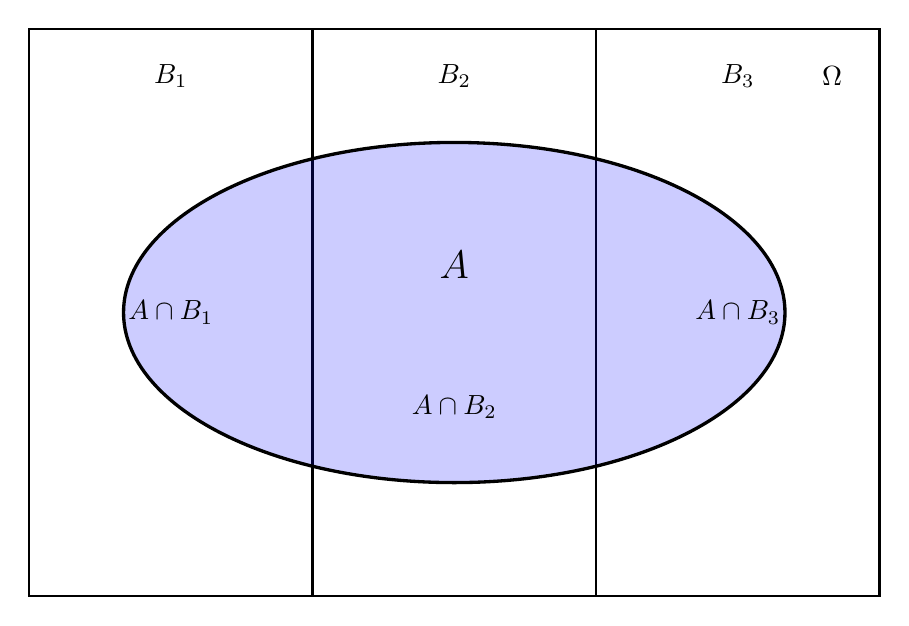
\begin{tikzpicture}[scale=1.2, thick]
    % Draw the sample space Omega
    \draw [line width=1pt] (0,0) rectangle (9,6);
    \node at (8.5, 5.5) {$\OmegaSet$};

    % Draw partitions
    \draw [line width=0.8pt] (3,0) -- (3,6);
    \draw [line width=0.8pt] (6,0) -- (6,6);

    % Label partitions
    \node at (1.5, 5.5) {$B_1$};
    \node at (4.5, 5.5) {$B_2$};
    \node at (7.5, 5.5) {$B_3$};

    % Draw Event A
    \draw [line width=1.2pt, fill=blue, fill opacity=0.2] (4.5, 3) ellipse (3.5cm and 1.8cm);
    \node[text=black, opacity=1] at (4.5, 3.5) {\Large $A$};

    % Label intersections
    \node[text=black, opacity=1] at (1.5, 3) {$A \cap B_1$};
    \node[text=black, opacity=1] at (4.5, 2) {$A \cap B_2$};
    \node[text=black, opacity=1] at (7.5, 3) {$A \cap B_3$};
\end{tikzpicture}
\end{center}
\vspace{0.5cm}

\subsection{Heuristics \& "Cheats"}
\begin{itemize}
    \item \textbf{The "Sequence" Cheat:} If a problem involves sequential stages (drawing from an urn, testing successively), immediately build a probability tree and apply the Law of Total Probability.
    \item \textbf{The "Rare Event" Cheat:} If the prevalence (prior) is $< 5\%$ and the test is imperfect, assume the Positive Predictive Value will be less than $50\%$. The base rate dominates!
\end{itemize}

\subsection{Pitfalls \& Fallacies}
\begin{itemize}
    \item \textbf{Prosecutor's Fallacy (Confusion of the Inverse):} Equating $\Pbb(A \mid B)$ with $\Pbb(B \mid A)$. Just because the probability of testing positive given you have cancer is $99\%$, does not mean the probability of having cancer given you test positive is $99\%$.
    \item \textbf{Affirming the Consequent (Logical Form):} If $A \implies B$, seeing $B$ does not imply $A$. Bayes' rule quantifies exactly \textit{how much} evidence $B$ actually provides for $A$.
    \item \textbf{Conditioning on Measure Zero:} Casually applying $\Pbb(A \mid B)$ when $\Pbb(B)=0$. In advanced measure theory, this requires the Borel-Kolmogorov paradox resolution and Radon-Nikodym derivatives.
\end{itemize}

\newpage
% ==============================================================================
\section{Part 5: Conceptual Synthesis and The "Big Picture"}
% ==============================================================================

\subsection{A) Thematic Connections}
The core thematic bridge here is \textbf{Invertibility in Asymmetric Information Systems}. In abstract algebra, we define inverse functions. In probability theory, Bayes' rule is the mathematical formulation of an inverse stochastic operator. It allows us to reverse the conditioning of random variables. If the underlying data generating process (DGP) dictates $Y \sim F(\cdot \mid X)$, Bayes' rule gives us the theoretical mapping to derive the distribution of $X \sim G(\cdot \mid Y)$.

\subsection{B) Forward and Backward Links}
\begin{itemize}
    \item \textbf{Backward Links:} This chapter logically extends basic axiomatic Set Theory and Combinatorics. We transition from "counting sets" to assigning continuous measures to $\sigma$-algebras and normalizing them under subsets (partitions).
    \item \textbf{Forward Links:} Understanding $\sigma$-algebra partitions is the absolute prerequisite for \textbf{Measure-Theoretic Conditional Expectation}, denoted $\Ebb[X \mid \Fcal_t]$. In advanced Stochastic Calculus, we don't condition on an event $B$, we condition on an entire sub-$\sigma$-algebra $\Fcal_t$ (the history of a process up to time $t$). Bayes' Rule natively scales to this via continuous conditional densities.
\end{itemize}

% ==============================================================================
\section{Part 6: Abstract Real-World Modeling (AI, ML, \& Quant Finance)}
% ==============================================================================

\subsection{A) Concrete Scenarios}
\begin{enumerate}
    \item \textbf{Algorithmic Trading (Hidden Markov Models):} A quantitative hedge fund wants to predict if the market is in a "Bull" or "Bear" regime (hidden states). They can only observe daily asset returns (noisy signals). Bayes' rule is used to iteratively update the probability of the market regime given the sequence of returns.
    \item \textbf{Generative AI (Diffusion Models / Variational Autoencoders):} In latent variable models, we have a complex data distribution $p(x)$ (e.g., images) and a latent prior $p(z)$. The neural network attempts to learn the intractable posterior $p(z \mid x)$ via Variational Inference, which is fundamentally grounded in Bayes' theorem.
\end{enumerate}

\subsection{B) Model Problem Setup: Quantitative Finance Regime-Switching Model}
Let us formalize the Algorithmic Trading scenario using a Bayesian filter.

\textbf{State Space & Probability Measure:} 
Let $(\OmegaSet, \Fcal, \Pbb)$ be our probability space. Let $X_t \in \{0, 1\}$ be the hidden market regime at time $t$ (0 = Bear, 1 = Bull). The state transitions follow a Markov Chain with transition matrix $P$, where $p_{ij} = \Pbb(X_t = j \mid X_{t-1} = i)$.
Let $Y_t \in \mathbb{R}$ be the observed daily return. The distribution of returns is conditionally Gaussian:
\[ Y_t \mid (X_t = j) \sim \mathcal{N}(\mu_j, \sigma_j^2) \]
Let $\Fcal_t^Y = \sigma(Y_1, \dots, Y_t)$ be the filtration generated by the observed returns up to time $t$. 

\textbf{The Objective:} Formulate the iterative Bayesian update for the belief vector $\pi_t = \Pbb(X_t = 1 \mid \Fcal_t^Y)$.

\begin{proof}[Formulation (The Bayesian Filter)]
We seek the posterior distribution $p(X_t \mid Y_{1:t})$. Using Bayes' theorem on continuous densities:
\[ p(X_t = j \mid Y_{1:t}) = \frac{f(Y_t \mid X_t = j) \Pbb(X_t = j \mid Y_{1:t-1})}{\sum_{i \in \{0,1\}} f(Y_t \mid X_t = i) \Pbb(X_t = i \mid Y_{1:t-1})} \]

The term $\Pbb(X_t = j \mid Y_{1:t-1})$ is the \textit{prior} at time $t$, derived from the Law of Total Probability applied to the Markov transition matrix:
\[ \Pbb(X_t = j \mid Y_{1:t-1}) = \sum_{k \in \{0,1\}} \Pbb(X_t = j \mid X_{t-1} = k) \Pbb(X_{t-1} = k \mid Y_{1:t-1}) \]
\[ = \sum_{k \in \{0,1\}} p_{kj} \pi_{t-1}^{(k)} \]

This yields a recursive stochastic difference equation for the trader's belief state, enabling dynamic portfolio weight optimization (e.g., via the Kelly Criterion) based strictly on Bayesian evidence updates.
\end{proof}

\newpage
% ==============================================================================
\section{Part 7: Common Variations and Untested Concepts}
% ==============================================================================

A glaring omission in the standard introductory problems is the \textbf{Continuous Form of Bayes' Theorem}, heavily used in Machine Learning and Bayesian Statistics.

\begin{theorem}[Continuous Bayes' Theorem]
Let $X$ and $Y$ be continuous random variables with joint probability density function (pdf) $f_{X,Y}(x,y)$. Let $f_X(x)$ and $f_Y(y)$ be the marginal pdfs. The conditional density of $X$ given $Y=y$ is:
\[ f_{X \mid Y}(x \mid y) = \frac{f_{Y \mid X}(y \mid x)f_X(x)}{\int_{-\infty}^{\infty} f_{Y \mid X}(y \mid x)f_X(x) \, dx} \]
\end{theorem}

\textbf{Worked Example: Bayesian Update of a Gaussian Prior.}
Suppose we are estimating an unknown parameter $\theta \sim \mathcal{N}(0, 1)$. We observe a noisy signal $x \mid \theta \sim \mathcal{N}(\theta, 1)$. Find the posterior distribution of $\theta \mid x$.

\begin{proof}[Derivation]
The prior is $f(\theta) \propto \exp(-\frac{\theta^2}{2})$.
The likelihood is $f(x \mid \theta) \propto \exp(-\frac{(x - \theta)^2}{2})$.
By Continuous Bayes:
\[ f(\theta \mid x) \propto f(x \mid \theta) f(\theta) = \exp\left(-\frac{1}{2} [(x - \theta)^2 + \theta^2] \right) \]
Expand the exponent:
\[ (x^2 - 2x\theta + \theta^2) + \theta^2 = 2\theta^2 - 2x\theta + x^2 = 2\left(\theta^2 - x\theta + \frac{x^2}{4}\right) + \frac{x^2}{2} = 2\left(\theta - \frac{x}{2}\right)^2 + \frac{x^2}{2} \]
Absorbing the terms independent of $\theta$ into the proportionality constant, we find:
\[ f(\theta \mid x) \propto \exp\left(-\frac{1}{2(1/2)} \left(\theta - \frac{x}{2}\right)^2 \right) \]
This mathematically proves the posterior is a new Gaussian: $\theta \mid x \sim \mathcal{N}\left(\frac{x}{2}, \frac{1}{2}\right)$. The variance has decreased from $1$ to $0.5$ (we have reduced our uncertainty through Bayesian updating).
\end{proof}

\newpage
% ==============================================================================
\section{Part 8: Advanced Diagnostic Testing: "Find the Flaw"}
% ==============================================================================

Act as the grader for the following five student submissions. Each contains a subtle, critical logical or mathematical flaw.

\subsection*{Problem 1: The Commutative Probability Proof}
\textbf{Student Proof:} We wish to evaluate $\Pbb(A \mid B)$. By the definition of conditional probability, $\Pbb(A \mid B) = \frac{\Pbb(A \cap B)}{\Pbb(B)}$. Since set intersection is commutative, $A \cap B = B \cap A$. Therefore, $\Pbb(A \mid B) = \frac{\Pbb(B \cap A)}{\Pbb(A)}$. Thus, $\Pbb(A \mid B) = \Pbb(B \mid A)$.

\subsection*{Problem 2: The Continuous Conditioning Trap}
\textbf{Student Proof:} Let $X \sim \text{Uniform}(0,1)$ and $Y = X^2$. We want to find $\Pbb(Y < 0.5 \mid X = 0.5)$. By definition, $\Pbb(Y < 0.5 \mid X = 0.5) = \frac{\Pbb(Y < 0.5 \cap X = 0.5)}{\Pbb(X = 0.5)}$. Since $\Pbb(X=0.5) = 0$ for a continuous random variable, the fraction is $0 / 0 = 0$, so the probability is zero.

\subsection*{Problem 3: The Independence Fallacy}
\textbf{Student Proof:} Let $A, B, C$ be mutually independent events. We want to find the probability of $A$ given $(B \cup C)$. 
\[ \Pbb(A \mid B \cup C) = \frac{\Pbb(A \cap (B \cup C))}{\Pbb(B \cup C)} \]
Because they are independent, $\Pbb(A \cap (B \cup C)) = \Pbb(A) \times \Pbb(B \cup C)$. 
So, $\Pbb(A \mid B \cup C) = \Pbb(A)$. Thus, any event is independent of the union of other independent events.

\subsection*{Problem 4: The Incomplete Partition}
\textbf{Student Proof:} A factory has machines A, B, and C producing 40\%, 40\%, and 10\% of the output respectively. Defect rates are 1\%, 2\%, and 3\%. 
To find the total probability of a defect $D$:
$\Pbb(D) = \Pbb(D \mid A)\Pbb(A) + \Pbb(D \mid B)\Pbb(B) + \Pbb(D \mid C)\Pbb(C) = (0.01)(0.4) + (0.02)(0.4) + (0.03)(0.1) = 0.004 + 0.008 + 0.003 = 0.015$. 
So the defect rate is $1.5\%$.

\subsection*{Problem 5: Sub-additivity as Additivity}
\textbf{Student Proof:} Let $A_1, A_2, \dots$ be an infinite sequence of events where $\Pbb(A_i) = \frac{1}{2^i}$. We want to find the probability of their union.
By Kolmogorov's axiom of additivity, $\Pbb\left(\bigcup_{i=1}^\infty A_i\right) = \sum_{i=1}^\infty \Pbb(A_i) = \sum_{i=1}^\infty \frac{1}{2^i} = 1$. The probability is exactly 1.

\vspace{1cm}
\hrule
\vspace{0.5cm}

\subsection*{Solution Key for the Grader}

\textbf{Flaw 1:} The student incorrectly swapped the denominator. While $A \cap B = B \cap A$ is true, $\frac{\Pbb(B \cap A)}{\Pbb(B)}$ does NOT equal $\frac{\Pbb(B \cap A)}{\Pbb(A)}$. The denominator must remain $\Pbb(B)$. They equated $\Pbb(B) = \Pbb(A)$ without justification.

\textbf{Flaw 2:} The definition $\Pbb(A \mid B) = \frac{\Pbb(A \cap B)}{\Pbb(B)}$ strictly requires $\Pbb(B) > 0$. For continuous variables, conditioning on a point requires evaluating limits or using conditional probability density functions $f_{Y \mid X}(y \mid x)$, not discrete limits that yield undefined $0/0$ states.

\textbf{Flaw 3:} The conclusion is surprisingly true, but the algebraic manipulation $\Pbb(A \cap (B \cup C)) = \Pbb(A) \times \Pbb(B \cup C)$ is not an axiom; it requires proof. The student must expand $A \cap (B \cup C) = (A \cap B) \cup (A \cap C)$ and apply independence, then inclusion-exclusion, to validate the factorization. Circularly assuming the union behaves as a scalar event bypasses the proof requirement.

\textbf{Flaw 4:} The provided probabilities $\Pbb(A)=0.4, \Pbb(B)=0.4, \Pbb(C)=0.1$ sum to $0.9$, NOT $1.0$. The set $\{A, B, C\}$ is not a valid partition of the sample space, so the Law of Total Probability cannot be applied. There is a missing 10\% of production unaccounted for.

\textbf{Flaw 5:} Kolmogorov's axiom of countable additivity strictly requires the sets $A_i$ to be \textit{pairwise disjoint}. The student did not state or prove that $A_i \cap A_j = \emptyset$. If they are not disjoint, one can only use Boole's Inequality (sub-additivity): $\Pbb(\bigcup A_i) \le \sum \Pbb(A_i)$.

\end{document}